\chapter{CHEMICAL COMPOSITION}
% !TEX root = hazy1.tex

\section{Overview}

The default solar composition is summarized in Table
\ref{tab:CompositionSolar}.  C and O abundances come from photospheric
abundances of \citet{Allende2002,Allende2001}, while N, Ne, Mg, Si,
and Fe are from \citet{Holweger2001}.  The helium abundance is a
typical value for nebulae with near-solar compositions.  The remainder
of the first thirty elements comes from \citet{Grevesse1998}.
Meteoritic and photospheric abundances agree for most elements.  They
differ by significant amounts for P, S, Cl, and Mn.  These are fairly
volatile elements so may be deficient in meteorites.  For these four
the means of the meteoritic and photospheric abundances were used.
The default solar abundances are stored in the file
\cdFilename{data/abundances/default.abn} and can be changed
by altering or overwriting that file.

These default abundances are maintained for backwards compatibility.
The \cdCommand{abundances GASS} command described 
in section \ref{sec:2010SolarComposition} will use values from 
\citet{Grevesse2010}.

\begin{table}
\centering
\caption{Default Solar Composition}
\label{tab:CompositionSolar}
\begin{tabular}{lllllll}
\hline
A&&&12+log& log& $n/n$(H)& ref\\
\hline
1& H& Hydrogen& 12.00& 0.00& 1.00E+00& GS98\\
2& He& Helium& 11.00& $-$1.00& 1.00E-01& text\\
3& Li& Lithium& 3.31& $-$8.69& 2.04E-09& GS98\\
4& Be& Beryllium& 1.42& $-$10.58& 2.63E-11& GS98\\
5& B& Boron& 2.79& $-$9.21& 6.17E$-$10& GS98\\
\hline
6& C& Carbon& 8.39& $-$3.61& 2.45E-04& AP02\\
7& N& Nitrogen& 7.93& $-$4.07& 8.51E-05& H01\\
8& O& Oxygen& 8.69& $-$3.31& 4.90E-04& AP01\\
9& F& Fluorine& 4.48& $-$7.52& 3.02E-08& GS09\\
10& Ne& Neon& 8.00& $-$4.00& 1.00E-04& H01\\
\hline
11& Na& Sodium& 6.33& $-$5.67& 2.14E-06& GS98\\
12& Mg& Magnesium& 7.54& $-$4.46& 3.47E-05& H01\\
13& Al& Aluminium& 6.47& $-$5.53& 2.95E-06& GS98\\
14& Si& Silicon& 7.54& $-$4.46& 3.47E-05& H01\\
15& P& Phosphorus& 5.51& $-$6.50& 3.20E-07& GS98*\\
\hline
16& S& Sulphur& 7.27& $-$4.74& 1.84E-05& GS98*\\
17& Cl& Chlorine& 5.28& $-$6.72& 1.91E-07& GS98\\
18& Ar& Argon& 6.40& $-$5.60& 2.51E-06& GS98\\
19& K& Potassium& 5.12& $-$6.88& 1.32E-07& GS98\\
20& Ca& Calcicum& 6.36& $-$5.64& 2.29E-06& GS98\\
\hline
21& Sc& Scandium& 3.17& $-$8.83& 1.48E-09& GS98\\
22& Ti& Titanium& 5.02& $-$6.98& 1.05E-07& GS98\\
23& V& Vanadium& 4.00& $-$8.00& 1.00E-08& GS98\\
24& Cr& Chromium& 5.67& $-$6.33& 4.68E-07& GS98\\
25& Mn& Manganese& 5.46& $-$6.54& 2.88E-07& GS98*\\
\hline
26& Fe& Iron& 7.45& $-$4.55& 2.82E-05& H01\\
27& Co& Cobalt& 4.92& $-$7.08& 8.32E-08& GS98\\
28& Ni& Nickel& 6.25& $-$5.75& 1.78E-06& GS98\\
29& Cu& Copper& 4.21& $-$7.79& 1.62E-08& GS98\\
30& Zn& Zinc& 4.60& $-$7.40& 3.98E-08& GS98\\
\hline
\end{tabular}\\[0.5pc]
References: GS98: \citet{Grevesse1998}, GS98* - mean of photospheric
and meteoritic, H01: \citet{Holweger2001}, AP01, AP02
\citet{Allende2001,Allende2002}.
\end{table}

Abundances are always specified by \emph{number} relative to
\emph{hydrogen,} not by mass or relative to silicon.
Abundances are relative to the total hydrogen
density, the sum of H in atomic, ionic, and molecular form.
These are gas-phase abundances
and do not include material locked into grains.
The
composition will be printed in the header information that starts the
printout.
You should check this to confirm that the right composition is
used.

The following sections describe how to modify the chemical composition.

\section{Absolute abundances and scale factors }

Abundances can be specified as either \emph{absolute abundances} or as
\emph{scale factors.}
An absolute abundance gives the abundance of an element relative
to hydrogen.
An example might be $n(\mathrm{O} ) /n( \mathrm{H} ) = 4 \times 10^{-4}$.
A relative abundance
is given relative to another value.
An example might be the abundance
relative to the solar value, $n(\mathrm{O}) / n(\mathrm{H}) = 4 \times
[n(\mathrm{O})/n(\mathrm{H})]_\odot$.

\section{Precedence}

There are many ways to specify an abundance.
It is even possible to specify different abundances for the
same element in the same input script.
If the absolute abundance is specified with more than one command then
the last abundance is used.
If the abundance is specified by both its
absolute abundance and by a scale factor then both are used.
Either of
the following will multiply the default \hii\ region nitrogen abundance by
a factor of two:
\begin{verbatim}
abundances H II region
element scale factor nitrogen 2
\end{verbatim}
or
\begin{verbatim}
element scale factor nitrogen 2
abundances H II region
\end{verbatim}
The \cdCommand{element scale factor} option applies a scale factor
while the
\cdCommand{element abundance} option sets an absolute abundance.
The \cdCommand{abundances \hii\ region}
command uses one of the absolute abundance mixtures that are stored
by the code.
This command enters the gas-phase
abundances of all \LIMELM\ elements and also includes interstellar grains.
The \cdCommand{element} command changes some details about a particular element.

In the following example both commands set absolute abundances so the
first nitrogen \cdCommand{abundance} will have no effect and the final nitrogen abundance
will be the default \hii\ region abundance
\begin{verbatim}
element abundance nitrogen -4.7
abundances H II region
\end{verbatim}
In the following only the second nitrogen scale factor has any
effect since the second scale factor overwrites the first:
\begin{verbatim}
element scale factor nitrogen 3
element scale factor nitrogen 2
abundances H II region
\end{verbatim}
The result will be \hii\ region abundances with nitrogen having twice its
normal value.
Similarly, the combination
\begin{verbatim}
element abundance nitrogen -4
element scale factor nitrogen 2
\end{verbatim}
in either order would result in
$n(\mathrm{N})/n(\mathrm{H}) = 2\times10^{-4}$ since the first command
sets an absolute abundance of $10^{-4}$ and the second command
doubles this.

The chemical composition is printed at the start of the calculation.
Be sure to confirm that the composition has been entered correctly.

\section{Abundances he c\dots}
\label{sec:CommandAbundances}

The abundances of all elements can be entered with the command
\cdCommand{abundances}
followed by:
a) a complete set of abundances,
b) the keyword \cdCommand{all} and
a single number to set all of the abundances,
or c) a second keyword to select
one of the stored abundance sets.

\subsection{Arbitrary abundances}

The \cdCommand{abundances} command can be used to specify the abundances of
a number of elements in one command.
The composition can be
specified on several lines with \cdCommand{continue} lines
following the initial \cdCommand{abundances} line.
Abundances of zero are not allowed; \Cloudy\ will stop if
they are entered.
Elements can be turned off with the \cdCommand{elements off} command.

The element symbol must be written before its abundance to identify
what element the value belongs to. An optional equals sign is allowed
in between the symbol and the value to improve readability.
The abundances can be entered in any order.

The best way to enter abundances is as \emph{absolute abundances},
as in the following example
\begin{verbatim}
abundances he =-1 li =-9   be =-11 b  =-9 c  =-4.3 n  =-5 o  =-2.3
continue    f =-7 ne =-1.2 na =-3  mg =-8
continue   al =-8 si =-8   p  =-6  s  =-8 cl =-9   ar =-8 k  =-6
continue   ca =-8 sc =-9   ti =-7  v  =-8 cr =-6.3 mn =-6 fe =-8
continue   co =-9 ni =-8   cu =-7  zn =-7
\end{verbatim}
The abundances can also be entered as a set of scale factors indicating
the desired abundances relative to the current set absolute abundance.
These will be solar by default.
The following example doubles the oxygen
abundance and lowers the iron abundance
\begin{verbatim}
abundances he =1 li =1 be =1 b  =1 c  =1 n  =1 o  =2
continue   f  =1 ne =1 na =1 mg =1
continue   al =1 si =1 p  =1 s  =1 cl =1 ar =1 k  =1
continue   ca =1 sc =1 ti =1 v  =1 cr =1 mn =1 fe =0.0000001 #deplete iron
continue   co =1 ni =1 cu =1 zn =1
\end{verbatim}
It is better to specify absolute abundances since the default solar
composition changes from time to time.

The code checks the sign of all of the entered abundances to decide
which style was entered.
The numbers are interpreted as linear scale factors
if \emph{all} are positive,
and as logs of the abundance relative to hydrogen if
\emph{any} are negative.

\subsection{Setting all at once}

If the keyword \cdCommand{all} appears and exactly one number
is entered then all
of the elements heavier than hydrogen are given this absolute abundance.
The number is the log of the abundance if it is less than or equal to zero
and the abundance itself if it is positive.
Either of the following commands
will give all elements between and including helium and zinc an absolute
abundance of $10^{-10}$ by number relative to hydrogen:
\begin{verbatim}
abundances all -10
abundances all 1e-10
\end{verbatim}
The \cdCommand{metals} command will set abundances
of all elements heavier than helium.

\subsection{Abundance ``filename.abn'' -- using tables of abundances}

A set of abundances stored in an external file are used if there are no numbers on the
\cdCommand{abundances} command but a file name 
occurs in quotation marks. 
The following gives some examples:
\begin{verbatim}
abundances "cameron.abn"
abundances "HII.abn" no grains
\end{verbatim}


Table \ref{tab:AbundanceSetsStored} lists some of the abundance sets
that are included in the distribution.
The keyword given in the first column of Table \ref{tab:AbundanceSetsStored}
can be used rather than the filename.  
This maintains compatibility with versions C13 and before.
This abundance sets in this table have been part of the code's distribution for a number of years
and more recent sets are not listed here.
Do a listing of the \cdFilename{*.abn} files in  \cdFilename{data/abundances}
to get a full list of the available abundances.

\begin{table}
	\small
	\centering
	\caption{Stored Abundance Sets}
	\label{tab:AbundanceSetsStored}\begin{tabular}{llp{6cm}l}
	\hline
	Keyword		& Filename			& Description					& grains? \\
	\hline
			& \cdFilename{default.abn}	& The default abundances				& no \\
	CAMEron		& \cdFilename{Cameron.abn}	& These are from \citet{Cameron1982}.			& no \\
	PRIMordial	& \cdFilename{primordial.abn}	& The primordial abundances.				& no \\
	CRAB		& \cdFilename{crab.abn}		& These are from model M1, Table 3, of
							  \citet{PequignotDennefeld1983}.			& no \\
	NOVA		& \cdFilename{nova.abn}		& These are roughly those derived by
							  \citet{Ferland1978}.					& no \\
	\hii, ORIOn	& \cdFilename{hii.abn}		& The \hii\ region abundances are the mean of the Orion
							  Nebula abundances given in three studies.		& Orion \\
	AGB, PLANetary	& \cdFilename{pn.abn}		& These abundances are from \citet{Aller1983} and
							  \citet{Khromov1989}, with high depletions assumed for
							  elements they do not list.				& ISM \\
	ISM		& \cdFilename{ism.abn}		& The gas-phase abundances are an average for the warm
							  and cold phases of the interstellar medium.		& ISM \\
	OLD SOLAR 84	& \cdFilename{solar84.abn}	& The composition will be the solar used in versions
							  84--94 of the code.  These are defined in Table
							  \ref{tab:CompositionSolarOld} and were taken from the
							  meteoritic abundances of \citet{Grevesse1989} with
							  extensions by \citet{Grevesse1993}.  All three of the
							  keywords \cdCommand{old solar 84} must appear.	& no \\
	GASS		& \cdFilename{solar\_GASS10.abn}& This will use solar abundances
							  \label{sec:2010SolarComposition} from
							  \citet{Grevesse2010}. The abundances are listed in
							  Table \ref{tab:2010SolarComposition}.			& no \\
	ALLEn		& \cdFilename{allen73.abn}	& These are the cosmic abundances of \citet{Allen1973}.	& no \\
	\hline
	\end{tabular}
\end{table}

Some of the stored abundance sets include grains, as indicated in Table \ref{tab:AbundanceSetsStored}.
The \cdCommand{no grains} and \cdCommand{no QHeat} options are recognized,
as described on the \cdCommand{grains} command (see section \ref{sec:GrainsCommand}).
For instance, ISM abundances but Orion grains would be specified with the combination
\begin{verbatim}
grains Orion
abundances "ISM.abn" no grains
\end{verbatim}
Because of the ability to use keywords, this is equivalent to
\begin{verbatim}
grains Orion
abundances ISM no grains
\end{verbatim}

The abundances files contain lines giving the name of an element and its abundance relative 
to hydrogen. 
Hydrogen may be in specified, or may not be.  If the abundance of hydrogen is 
given and is not equal to unity the code will rescale the abundances by the entered value 
for hydrogen.  If hydrogen is not specified it is assumed to have an abundance
of 1.

All elements heavier than hydrogen are turned off before the abundance files are read.
An element is turned on if it appears in the file.
If an element is not included in the file it will not be included in the calculation.

The \cdCommand{abundances} command has a \cdCommand{print} option to report
grain types and abundances entered for each active element.

\subsection{Abundance available}

You can obtain a list of all the abundance files that are present on the search
path using the \cdCommand{abundance available} command. This will include
user-installed abundance files by simply listing all files with names ending with \cdFilename{.abn}.
It is not possible to check whether these files actually contain a valid abundance table.
This command will exit immediately after printing the list.

\subsection{Older solar abundances}

The default solar abundances are stored in the file 
\cdFilename{data/abundances/solar.abn} and can be changed
by altering or overwriting that file.

The keyword \cdCommand{old solar 84} uses the solar composition
used in versions 84 - 94 of the code.
These are defined in Table \ref{tab:CompositionSolarOld}
and were taken from the
meteoritic abundances of \citet{Grevesse1989} with extensions by
\citet{Grevesse1993}.
The keyword \cdCommand{Cameron} uses the \citet{Cameron1982}
abundances.
The keyword \cdCommand{Allen} uses the \citet{Allen1973} abundances.
These are maintained for historical reasons.

\begin{table}
\centering
\caption{Old Solar Composition, default in versions C84 - C94}
\label{tab:CompositionSolarOld}
\begin{tabular}{llllll}
\hline
&&&&Solar\\
\hline
1& H& Hydrogen& 1& 0.00& 12.00\\
2& He& Helium& 0.1& $-$1.00& 11.00\\
3& Li& Lithium& 2.04E-09& $-$8.69& 3.31\\
4& Be& Beryllium&  2.63E-11& $-$10.58&1.42\\
5& B& Boron&  7.59E-10& $-$9.12&2.88\\
\hline
6& C& Carbon&  3.55E-04&$-$3.45& 8.55\\
7& N& Nitrogen& 9.33E-05& $-$4.03& 797\\
8& O& Oxygen& 7.41E-04& $-$3.13& 8.87\\
9& F& Fluorine& 3.02E-08&  $-$7.52&4.48\\
10& Ne& Neon& 1.17E-04& $-$3.93& 8.07\\
\hline
11& Na& Sodium& 2.06E-06& $-$5.69& 6.31\\
12& Mg& Magnesium& 3.80E-05& $-$4.42& 7.58\\
13& Al& Aluminium& 2.95E-06& $-$5.53& 6.47\\
14& Si& Silicon& 3.55E-05& $-$4.44& 7.55\\
15& P& Phosphorus& 3.73E-07& $-$6.43& 5.57\\
\hline
16& S& Sulphur& 1.62E-05& $-$4.79& 7.21\\
17& Cl& Chlorine& 1.88E-07& $-$6.73& 5.27\\
18& Ar& Argon& 3.98E-06& $-$5.40& 6.60\\
19& K& Potassium& 1.35E-07& $-$6.87& 5.13\\
20& Ca& Calcicum&  2.29E-06&$-$5.64& 6.36\\
\hline
21& Sc& Scandium&  1.58E-09&  $-$8.80& 3.20\\
22& Ti& Titanium&  1.10E-07& $-$6.96& 5.04\\
23& V& Vanadium& 1.05E-08& $-$7.98& 4.02\\
24& Cr& Chromium&  4.84E-07& $-$6.32& 5.68\\
25& Mn& Manganese& 3.42E-07& $-$6.47& 5.53\\
\hline
26& Fe& Iron& 3.24E-05& $-$4.49& 7.51\\
27& Co& Cobalt&  8.32E-08& $-$7.08& 4.92\\
28& Ni& Nickel&  1.76E-06& $-$5.75& 6.25\\
29& Cu& Copper& 1.87E-08& $-$7.73& 4.27\\
30& Zn& Zinc& 4.52E-08& $-$7.34& 4.66\\
\hline
\end{tabular}
\end{table}

\begin{table}
\centering
\caption{2010 Solar Composition, keyword \protect\cdCommand{GASS}}
\label{tab:2010SolarComposition}
\begin{tabular}{lllll}
\hline
&&&Solar\\
\hline
1& H& 1& 0& 12\\
2& He& 8.51E-02& -1.07& 10.93\\
3& Li& 1.12E-11& -10.95& 1.05\\
4& Be& 2.40E-11& -10.62& 1.38\\
5& B& 5.01E-10& -9.3& 2.7\\
6& C& 2.69E-04& -3.57& 8.43\\
7& N& 6.76E-05& -4.17& 7.83\\
8& O& 4.90E-04& -3.31& 8.69\\
9& F& 3.63E-08& -7.44& 4.56\\
10& Ne& 8.51E-05& -4.07& 7.93\\
11& Na& 1.74E-06& -5.76& 6.24\\
12& Mg& 3.98E-05& -4.4& 7.6\\
13& Al& 2.82E-06& -5.55& 6.45\\
14& Si& 3.24E-05& -4.49& 7.51\\
15& P& 2.57E-07& -6.59& 5.41\\
16& S& 1.32E-05& -4.88& 7.12\\
17& Cl& 3.16E-07& -6.5& 5.5\\
18& Ar& 2.51E-06& -5.6& 6.4\\
19& K& 1.07E-07& -6.97& 5.03\\
20& Ca& 2.19E-06& -5.66& 6.34\\
21& Sc& 1.41E-09& -8.85& 3.15\\
22& Ti& 8.91E-08& -7.05& 4.95\\
23& V& 8.51E-09& -8.07& 3.93\\
24& Cr& 4.37E-07& -6.36& 5.64\\
25& Mn& 2.69E-07& -6.57& 5.43\\
26& Fe& 3.16E-05& -4.5& 7.5\\
27& Co& 9.77E-08& -7.01& 4.99\\
28& Ni& 1.66E-06& -5.78& 6.22\\
29& Cu& 1.55E-08& -7.81& 4.19\\
30& Zn& 3.63E-08& -7.44& 4.56\\
\hline
\end{tabular}
\end{table}

\subsection{Grains, gas-phase depletions, and quantum heating}

Certain elements, especially Si, Ca, Al, Mg, and Fe,
are heavily depleted
onto grains in the ISM.
\citet{KingdonFerlandFeibelman1995} discuss the observational
effects of grains upon an \hii\ region.
The abundance sets specified by the
\cdCommand{H II region},
\cdCommand{ISM}, or \cdCommand{planetary nebula} keywords
will include grains and the gas-phase
mixtures given in Table \ref{tab:AbundanceSetsStored}.
The bottom line of the table lists the type
of grains that are included by default.
These types are defined in the section on grains
starting on page \pageref{sec:GrainsCommand}.

Grains can also be specified separately with the
\cdCommand{grains} command (see section \ref{sec:GrainsCommand}).
If you use the \cdCommand{grains} command to specify another type
of grains then you should include the keyword
\cdCommand{no grains} on the abundances
line to prevent the default grains from also being used.

If you set the keyword \cdCommand{no grains} to not include
the default grains and
do not specify another set of grains with the
\cdCommand{grains} command then grains
will not be included in the calculation but the depleted
gas-phase abundances
will still be used.\footnote{In versions 77 and before,
the abundances of depleted elements were
set to solar values when \cdCommand{no grains} was set.}
This is, of course, not self-consistent.

Quantum or single-photon heating will be considered for all
grain species where it will be important.
Quantum heating only affects the Wien tail of the grain
thermal-emission spectrum but is computationally fairly expensive.
The \cdCommand{no qheat} option on the \cdCommand{abundances} command
will disable quantum heating.
Figure \ref{fig:grains_qheat} compares the continuum predicted
in the test case \cdFilename{grains\_qheat},
a part of the code's test suite.
Quantum heating is normally
included and the \cdCommand{no qheat} option was used to
disable it to make this comparison.

To access the full range of grain options it is best to combine the \cdCommand{no grains}
option on the \cdCommand{abundances} command and follow that with
the \cdCommand{grains} command and its options,
described in section \ref{sec:GrainsCommand}), as in
\begin{verbatim}
abundances ISM no grains
grains [options]
\end{verbatim}

\begin{figure}
\centering
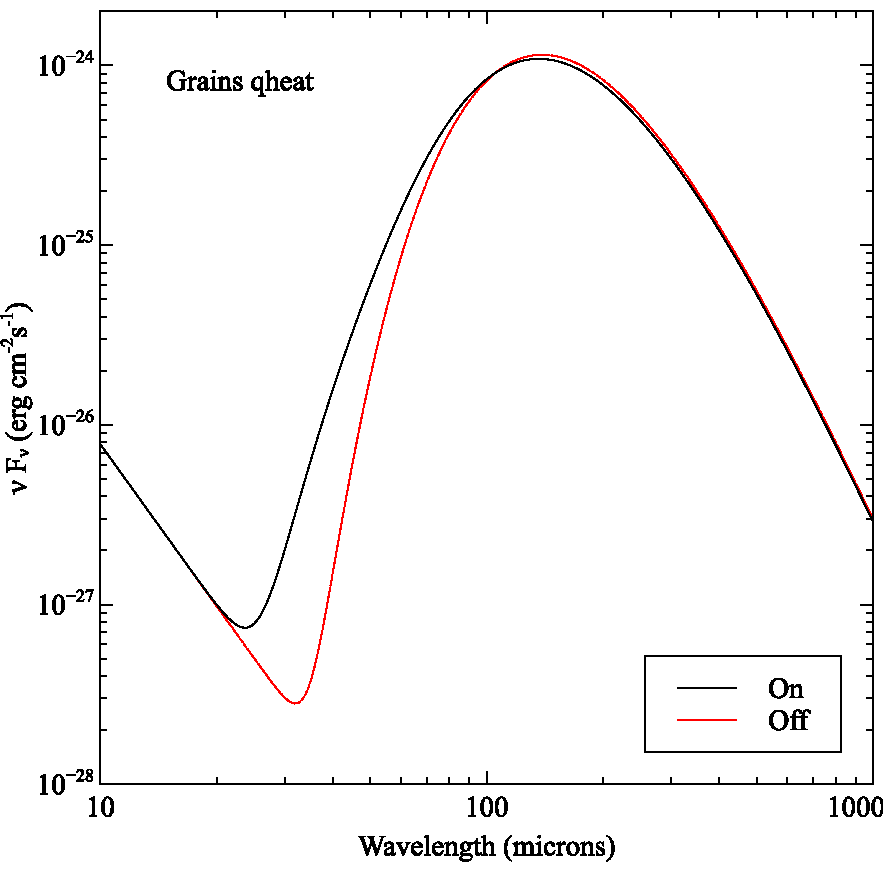
\includegraphics{grains_qheat}
\caption[Quantum heating]{\label{fig:grains_qheat}This figure shows the
net emission computed by the test case
\cdFilename{grains\_qheat.}
The solid line includes quantum heating while the dashed
line has disabled~it. The emission lines have been suppressed in this plot for clarity.}
\end{figure}
% this figure generated with the docs/latex/hazy1/grains_qheat* files
% grains_qheat.in was from tsuite/auto at time of this revision
% run both grains_qheat*.in files, open Veusz file grains_qheat.vsz
% and update data to regenerate Figure.  Export to
% grains_qheat.pdf to update figure in Hazy1

\subsection{Interactions between the abundances and grains commands}

It is possible to include grain species with both the
\cdCommand{abundances} command,
described here, and with the \cdCommand{grains} command.
For simplicity you should only set the grain abundances
only once.
If you specify the same grains more than one time you are asking
for trouble.
The rules for how these commands interact are described elsewhere.

You should check that you have the expected grain abundances by looking
at the list of grain abundances given at the start of the calculation and
at the value of $A_V/N_{\mathrm{H}}$ given at the end.

\section{Abundances starburst, Z=10}

This form of the \cdCommand{abundances} command interpolates on
Fred Hamann's grid
of abundances for an evolving starburst in a massive galactic core.
The
chemical evolution model is more fully described by \citet{Hamann1993}.
This grid is model M5a of that paper.
It uses a star formation
rate and infall timescales very close to, but slightly faster than,
the
``standard'' elliptical model (see also \citealp{Arimoto1987,Matteucci1986,Matteucci1987,Bica1988}).
Its IMF also
has a slope very similar to, but slightly steeper than
($x = 1.0$ instead of 1.1), that of the standard elliptical model.
The main difference is
that the IMF has a lower mass cutoff at $M = 2.5 M_\odot$ instead of
$\sim 0.1 M_\odot$ in the standard models.
This allows the gas to reach much higher metallicities
before the gas is locked up in low-mass stellar remnants.

The metallicity of the gas relative to solar appears on the line.
It is interpreted as the log of the metallicity if it is
less than or equal
to zero, and the linear metallicity if positive.
The keywords
\cdCommand{log} or \cdCommand{linear}
will force the number to be interpreted appropriately.
The limits to the
range of possible metallicities are $10^{-3} Z_{sun}$ and $36 Z_{sun}$.

This command works by generating scale factors that multiply
the current standard abundance.
This is solar by default.
The command does not derive
absolute abundances.
If you change the abundances with a second
\cdCommand{abundance}
command then the scale factors will multiply those new abundances.

The keyword \cdCommand{trace} will print the abundances of
all elements as a function
of metallicity between the full $10^{-3} Z_{sun}$ and
$36 Z_{sun}$ limits.
The code will then stop.

\section{Abundances isotopes}

Isotope fractions may be specified with this command by providing
one of the keywords entered in Table~\ref{tab:isotopes}, or a
filename enclosed in double-quotations.
Note that all tables rely on the \citet{Rosman1998}
terrestrial abundances for many isotopes.
For instance, \citet{Asplund2009} make use of the
``representative isotopic composition'', while \citet{Lodders2003}
opts for the ``best measurement from a single terrestrial source''.
By default, the abundances of \citet{Asplund2009} are used,
modified to match the primordial D/H ratio of $1.65 \times 10^{-5}$
(\citealp{Pettini2001}), and to reproduce Cloudy's historic 13C isotope
fraction of 1/30.

\begin{table}
\centering
\caption{Isotope Fractions Data}
\label{tab:isotopes}
\begin{tabular}{llll}
\hline
Keyword		& Filename		& Abundance Type	&	Reference		\\
\hline
aspl		& ``Asplund09-iso.abn''	& Protosolar		&	\citet{Asplund2009}	\\
lodders09	& ``Lodders09-iso.abn''	& Protosolar		&	\citet{Lodders2009}	\\
lodders03	& ``Lodders03-iso.abn''	& Solar System		&	\citet{Lodders2003}	\\
rosm		& ``Rosman98-iso.abn''	& Terrestrial 		&	\citet{Rosman1998}	\\
    		& ``default-iso.abn''	& aspl + D/H + f(13C)	&				\\
\hline
\end{tabular}
\end{table}

Additional isotopic data used internally include masses
derived from \citet{Audi1995}, and spins and magnetic
moments obtained from \citet{Stone2005}.

Note that the command automatically resets the Deuterium
and 13C abundances.
The command \cdCommand{element name isotopes}, described
below, should be issued to maintain a desired isotope ratio,
following all instances of \cdCommand{abundances isotopes}.

A user-defined file must include fractions for all
the isotopes present in the default files.

\par
The default isotope abundances were used in our predictions
for hyperfine structure line emission from hot and rarefied
media, e.g., the intracluster medium in galaxy clusters, and
the Orion million K gas; these are discussed in detail in
\citet{Chatzikos2014}.

\section{Element name [scale, abundance, isotopes, off, log, table]}

This sets the abundance of a particular element.
The command has several
keywords that change the behavior of the command.

\subsection{Element name scale}

If the keyword \cdCommand{scale} appears
then the number on the line is a scale factor
multiplying the current abundance of the element.
The number is a linear
scale factor if it is positive or if the \cdCommand{linear}
keyword appears and it is
the log of the scale factor if the number is negative.
If the key \cdCommand{log}
appears (note the leading space) then the scale factor
is interpreted as
a log irregardless of its sign.

\subsection{Element name abundance}

If \cdCommand{abundance} appears then the number is
the absolute abundance of the
element by number relative to hydrogen.
The number is the log of the
abundance unless the \cdCommand{linear} keyword appears.

\subsection{Element name isotopes}

If the keyword \cdCommand{isotopes} appears, then
the code expects a pair of numbers, the atomic mass
number and the isotope fraction, for each of the
elemental isotopes.
Linear numbers are expected.

\subsubsection{Setting the D/H ratio}

This command should be used to set the D/H abundance ratio.
For example, the following sets the ratio to $2\times 10^{-5}$,
close to the current solar-system value:
%
\begin{verbatim}
element hydrogen isotopes (1, 1) (2, 2e-5)
\end{verbatim}

This mainly affects HD cooling.
The default is the primordial abundance of $1.65 \times 10^{-5}$
as measured by \citet{Pettini2001}.

The command \cdCommand{set D/H} has been deprecated.

\subsubsection{Setting the 12C/13C ratio}

This command should be used to set the 12C/13C ratio.
For instance, the following sets the ratio to 5:
%
\begin{verbatim}
element carbon isotopes (12, 5) (13, 1)
\end{verbatim}
%

The code currently predicts the $^{13}$CO rotation spectrum
and the intensity of
$^{13}\ciii\ \lambda 1910$\AA\ (\citealp{Clegg1997}) using this ratio.
The code does not now solve
for $^{12}$C and $^{13}$CO abundances and ionic fractions
but rather assumes that
the ratio $^{12}$CO/$^{13}$CO and the
$^{12}$C$^{+2}/^{13}$C$^{+2}$ ionization fractions are equal to
$^{12}$C/$^{13}$C.
This ignores chemical fractionation.
A full treatment of this physics is high on the list of priorities.

The $^{12}$C/$^{13}$C ratio depends on both location in the
galaxy and age.
It is $\approx 90$ in the solar system (\citealp{Asplund2009})
and reflects the galactic value when the sun formed.
The value toward the Galactic center
is about 20 increasing to $\approx77$ at the solar radius
(\citealp{Wilson1994}).
The default value of 30 is a compromise.

The command \cdCommand{set 12C13C} has been deprecated.

\subsection{Element isotopes all}

This command enables the available isotopologues of all molecules.
Currently, only singly-substituted isotopologues are available in
Cloudy.
Densities are simply scaling by fractionations of constituent elements.

Deuterium is not presently enabled by this command.
Isotopes of all other elements are enabled.

The command \cdCommand{set isotopes all} has been deprecated.

\subsection{Element name ionization }

This allows the ionization distribution of an element to be set.
Each
number is the ionization fraction, $n(A^{+i})/n(A)$,
for successive stages of
ionization.
The code will scan off up to A+1 numbers, where A is the atomic
number of the element.
If any numbers are negative then all are interpreted
as logs of the ionization fraction.
If there are fewer than A+1 numbers
then the missing stages of ionization are assumed to have zero abundance.

The total density of all ions must add up to the total density of the element.
The code imposes several particle conservation rules to insure that
mass is conserved.
The density of the ions will be renormalized so that the
total abundance of the element is equal to the value
specified by other commands.\footnote{In versions C08 and before this
command did not confirm that the sum of the ionization fractions
was unity.  The abundance of each stage of ionization was set to the product
of the ionization fraction times the abundance set by other commands.  If the
fractions did not add up to unity the effect was to change the total
abundance of the element.}

This command does not specify the chemical state.
The \htwo\ fraction can
be set with the \cdCommand{set H2} command.
Chemistry is disabled if you set the ionization distribution of an element
that is part of the chemical network.
It will not be possible to obtain
a chemical solution if the abundances of the atom and ions cannot respond
to changes in the chemistry.

All of this is unphysical and is only intended as a way to test the code.

\subsection{Element name off}

If the keyword \cdCommand{off} appears
(note the leading space) then the element
is not included in the calculation.
The ionization equilibrium, opacity,
and cooling due to the element will not be computed.

The keyword \cdCommand{on} will include an element that was
previously turned off in the same input stream.

You can save computer time if you turn an element off.
This is especially
true for third- and fourth-row elements.
These take longer to compute
because of the large number of inner-shell electrons.
They often have
negligible effects on the thermal and ionization structure because of
their low abundances.

Memory for the species that are present is dynamically allocated when
the code starts.
When the code is used to compute a large grid of models
it is not possible to turn on an element that was turned off for the first
model since the needed memory does not exist.
You can turn off an element
in later models since the element is simply not computed.
In later
calculations in a grid the code will ignore any attempt to turn on an
element that was initially turned off.

The chemical solution may become destabilized if an element that forms
molecules is turned off.
Do not turn off elements that are part of the
chemistry if the calculation extends into a PDR or molecular cloud.
The
code will generate a warning if this is done.

Turning off an element with this command has other side effects.
For instance, the following input stream would produce unexpected results:
\begin{verbatim}
element zinc ionization -3 0 -4
init "ism.ini"
element zinc on
\end{verbatim}
because the \cdFilename{ism.ini} file turns off zinc.
This destroys the memory of the
\cdCommand{element zinc ionization} command,
which sets the ionization of the element.
So, when the element is turned back on with the
\cdCommand{element zinc on} command
the ionization will be determined self consistently rather than set to the
constant values.

\subsection{Element limit off -12}
\label{sec:ElementLimitOffCommand}

\noindent Elements with abundances that are
smaller than the number on the line will be ignored.
The number is the log of the limiting abundance by number relative to
hydrogen.
This is an easy way to turn off elements that have trivial
abundances.
Table \ref{tab:CompositionDecreasingOrder} lists the elements
in terms of decreasing abundance.
The command
\begin{verbatim}
elements limit off -7
\end{verbatim}
would cause all elements at Cobalt and above in
Table \ref{tab:CompositionDecreasingOrder} to be turned off.

\begin{table}
\centering
\caption{Solar composition sorted by abundance}
\begin{tabular}{llll}
\hline
\label{tab:CompositionDecreasingOrder}
A& Symbol& Name& log $n(x)/n(\mathrm{H})$\\
4& Be& Beryllium& -10.58\\
5& B& Boron& -9.21\\
21& Sc& Scandium& -8.83\\
3& Li& Lithium& -8.69\\
23& V& Vanadium& -8.00\\
29& Cu& Copper& -7.79\\
9& F& Fluorine& -7.52\\
30& Zn& Zinc& -7.40\\
27& Co& Cobalt& -7.08\\
22& Ti& Titanium& -6.98\\
19& K& Potassium& -6.88\\
17& Cl& Chlorine& -6.72\\
25& Mn& Manganese& -6.54\\
15& P& Phosphorus& -6.50\\
24& Cr& Chromium& -6.33\\
28& Ni& Nickel& -5.75\\
11& Na& Sodium& -5.67\\
20& Ca& Calcium& -5.64\\
18& Ar& Argon& -5.60\\
13& Al& Aluminium& -5.53\\
16& S& Sulphur& -4.74\\
26& Fe& Iron& -4.55\\
12& Mg& Magnesium& -4.46\\
14& Si& Silicon& -4.46\\
7& N& Nitrogen& -4.07\\
10& Ne& Neon& -4.00\\
6& C& Carbon& -3.61\\
8& O& Oxygen& -3.31\\
2& He& Helium& -1.00\\
1& H& Hydrogen& 0.00\\
\hline
\end{tabular}
\end{table}

\subsection{Element name table}

If the keyword \cdCommand{table} appears on
the \cdCommand{elements} command then the code
will read in a list of position-dependent abundances for
a particular element.
This might, for instance, be used to model variable depletions.
The following is an example.
\begin{verbatim}
element carbon table depth
-30 -4
3 -4
5 -3
7 -2
9 -1
end of table
\end{verbatim}

The first number on each line is the log of the radius (the default)
or depth (if the keyword \cdCommand{depth} also appears
on the \cdCommand{element} line).
The second number is the
log of the abundance of the element at that point, by number relative to
hydrogen.
The table ends with a line starting with the keyword
\cdCommand{end}.
At least two pairs of data need to be entered to enable interpolation by the code.
There is no upper limit to the number of pairs that may be entered.
This command always specifies the absolute
abundance and not the scale factor.

The chemical composition printed at the start of the calculation is always
the composition at the illuminated face of the cloud.  If the table gives
composition as a function of radius then the composition will be evaluated
at the inner radius of the cloud.  If the table gives the composition as
a function of depth then the composition will be evaluated as a depth of
$10^{-30}$~cm.  The table must extend to this depth as in the example above.

\section{Fluctuations abundances, period, max, min, phase}
\label{sec:FluctuationsAbundanceCommand}

This makes the metallicity vary with radius as a sine wave.  This is
designed to investigate the effects of chemical inhomogeneities upon the
emission-line spectrum and was implemented to search for solutions to the
$t^2$ problem (\citealp{KingdonFerland1995}).

The first number is the log of the period $P$ of the sine wave in
centimeters.
The second two numbers are the logs of the largest and smallest
metallicities over the sine wave and have the same effect as the metals
scaling factor entered with the \cdCommand{metals} command.

The \cdCommand{fluctuations} command is more fully described in
Section \ref{sec:FluctuationsDensityCommand} on the density version.

\section{Grains}
\label{sec:GrainsCommand}

This command controls how grains are included in the calculation.
They are not included by default.
Grains are included in the compositions set
by some \cdCommand{abundances} commands
(see Table \ref{tab:AbundanceSetsStored} above).
Grain physics
was originally developed in collaboration with
Peter van Hoof, Peter G. Martin, and
Joe Weingartner. Peter van Hoof did the majority of the coding,
and he is the maintainer of the code.
Reviews are given by \citet{Spitzer1948,Spitzer1978}, and \citet{Martin1979}.
\citet{Baldwin1991},
\citet{Weingartner2001b}, \citet{VanHoof2004} and
\citet{Weingartner2006} describe the theory incorporated in the code.

The \cdCommand{save grain} commands produce
output giving details about the grains.
Some details of the grain physics
can be adjusted with the \cdCommand{no grain \dots} family of commands.
The \cdCommand{compile grains} command
(page \pageref{sec:CompileGrains} below) is used to 
create new grain opacity files, or to recompile them if
the code's energy mesh is changed.

\subsection{Using the built-in grain types}

The grain types summarized in Table \ref{tab:GrainStandardTypes} are
included in the code's data files.
The table gives the grain material, its size distribution,
and the name of the grain opacity file that it uses.
In most cases these
will be sufficient - nothing more needs to be done to set up the grains.

\begin{table}
\centering
\caption{Standard Grain Types}
\label{tab:GrainStandardTypes}
\begin{tabular}{llll}\hline
Keyword&Filename& Type& Size distribution\\
\hline
                                   & \cdFilename{graphite\_0m010.opc}& Graphite& Single 0.01 $\mu$m\\
                                    & \cdFilename{graphite\_0m100.opc}& Graphite& Single 0.1 $\mu$m\\
                                   & \cdFilename{graphite\_1m000.opc}& Graphite& Single 1 $\mu$m\\
ISM single graphite& \cdFilename{graphite\_ism\_01.opc}& Graphite& Unresolved ISM\\
ISM graphite            & \cdFilename{graphite\_ism\_10.opc}& Graphite& ISM, 10 bins\\
Orion single graphite& \cdFilename{graphite\_orion\_01.opc}& Graphite& Unresolved Orion\\
Orion graphite        & \cdFilename{graphite\_orion\_10.opc}& Graphite& Orion, 10 bins\\
grey single                         & \cdFilename{grey\_ism\_01.opc}& Grey& Unresolved ISM\\
grey                          & \cdFilename{grey\_ism\_10.opc}& Grey& ISM, 10 bins\\
PAH single              & \cdFilename{pah1\_ab08\_01.opc}& PAH& Unresolved AB08\\
PAH                          & \cdFilename{pah1\_ab08\_10.opc}& PAH& AB08, 10 bins\\
                                  & \cdFilename{pah1\_c120.opc}& PAH& 120 C atoms\\
                                  & \cdFilename{pah1\_c15.opc}& PAH  & 15 C atoms\\
                                  & \cdFilename{silicate\_0m010.opc}& Silicate& Single 0.01 $\mu$m\\
                                  & \cdFilename{silicate\_0m100.opc}& Silicate& Single 0.1 $\mu$m\\
                                  & \cdFilename{silicate\_1m000.opc}& Silicate& Single 1 $\mu$m\\
ISM single silicate& \cdFilename{silicate\_ism\_01.opc}& Silicate& Unresolved ISM\\
ISM silicate             & \cdFilename{silicate\_ism\_10.opc}& Silicate& ISM, 10 bins\\
Orion single silicate& \cdFilename{silicate\_orion\_01.opc}& Silicate& Unresolved Orion\\
Orion silicate          & \cdFilename{silicate\_orion\_10.opc}& Silicate& Orion, 10 bins\\
\hline
\end{tabular}
\end{table}

Grains are composed of elements that are condensed from the gas phase.
It would be inconsistent to assume solar abundances for all elements and
also include grains.
In reality certain elements, especially Ca, Al, Ti,
and Fe, are strongly depleted from the gas phase in the ISM
and are believed to be present as grains.
The \cdCommand{metals deplete} command can be used
to deplete elements that are included in grains.

Several of the standard abundance sets that are specified with the
\cdCommand{abundances} command include grains.
The elements which make
up the grains are depleted from the gas phase in these abundance sets.
Elements are not depleted in sets that do not include grains by default.

\begin{itemize}
\item \cdCommand{grains ISM}  specifies grains
with a size distribution
and abundance appropriate for the ISM of our galaxy.
This includes both a graphitic and
silicate component and generally reproduces the observed overall
extinction
properties for a ratio of extinction per reddening of
$R_V \equiv A_v/E(B-V) = 3.1$.
This is the default and will be used if no keywords occur on the
\cdCommand{grains} command.
If either keyword \cdCommand{graphite} or \cdCommand{silicate} also
appears then only that grain type is included.
Both species are included if neither keyword appears.

\item \cdCommand{grains Orion}
specifies graphitic and silicate grains with a size distribution and
abundance appropriate for those along the line of sight to the Trapezium
stars in Orion.
The Orion size distribution is deficient in small particles
and so produces the relatively grey extinction observed in
Orion (\citealp{Baldwin1991}).
If either keyword \cdCommand{graphite} or \cdCommand{silicate} appears
then only that grain type is included.
Both species are included if neither keyword appears.

\item \cdCommand{grains PAH} turns on PAHs.
See section \ref{sec:GrainPAHcommands} below for more details.
\end{itemize}

\cdTerm{Grain abundances}  An optional scale factor
on the command line changes
the grain abundance relative to its default value.
If the keyword \cdCommand{log}
appears or if the number is less than or equal to zero
then the number is the log of the scale factor.
It is the linear factor if the keyword linear
appears or if no keyword appears and the number is positive.

It is also possible to change the abundances of the grains with the
\cdCommand{metals grains} command.
The \cdCommand{metals} command scales the
abundances of all elements more massive than helium by a scale factor.
If the keyword \cdCommand{grains} occurs then the grain abundance
will also be scaled up or down.
This would keep the grains to metals abundance ratio constant.

The following example uses ISM gas-phase abundances, Orion silicates
with dust to gas ratio twice the default value,
and ISM graphite with default ISM abundances.
\begin{verbatim}
# use ISM abundances but DO NOT include ISM default grains
abundances ISM no grains
# Orion silicate with twice the Orion abundance
grains Orion silicate 2
# ism graphite with ISM dust to gas ratio
grains ISM graphite
\end{verbatim}
The default \hii\ region grain abundances are close to the ISM value.
Planetary nebula grain abundances are quite uncertain.
\citet{Clegg1989} find dust-to-gas ratios below the ISM value, while
\citet{Borkowski1991} find a dust-to-gas ratio an order of magnitude above ISM
in a hydrogen-deficient planetary nebula.
\citet{Mallik1988} find
dust-to-gas ratios roughly equal to the ISM in a sample of PNs.
\citet{Stasinska1999} discuss properties of a sample of PNe.
In view of this
scatter the grain abundance of PNe should probably be treated as a free
parameter.

\emph{Size resolved or averaged grains} Grains in the ISM have a
broad range of sizes, often described by a power-law distribution
(\citealp{Mathis1977}).
By default the grains will be resolved into ten size bins.
If the keyword \cdCommand{single} appears then the grains will have
properties determined
by averaging over the entire size range.
If the keyword \cdCommand{distribution} appears
then the code will resolve the size distribution.
This is the default and will be used if no keyword appears.
The \cdCommand{single} option may save some machine
time but will give a less realistic representation of the grain physics.
This is because many grain properties such as temperature and charge
depend strongly on the size.
In particular, the photoelectric heating of the gas
can be underestimated if the single mean grain is used.

\subsection{Interactions between abundances and grains commands}

Be careful when specifying grains with more than one
\cdCommand{grains} command or
with both the \cdCommand{abundances} and \cdCommand{grains} commands.
The order in which the
commands appear in the input stream does make a difference.
These commands
have the following precedence:

%%need bullet here
\begin{itemize}
\item An \cdCommand{abundance} command will override all grains set with a previous
\cdCommand{abundances} command.  So with the following pair
\begin{verbatim}
abundances ism
abundances old solar 84
\end{verbatim}
ISM grains stay in place since grains are not included in the
old solar mixture.
\begin{verbatim}
abundances ism
abundances orion
\end{verbatim}
only Orion grains will be included

\item An \cdCommand{abundances} command will NOT override any grains set
with a previous \cdCommand{grains} command.
It will not add any grains either.
Instead it will implicitly behave as if the option
\cdCommand{no grains}
was given on the \cdCommand{abundances} command.
\begin{verbatim}
grains orion
abundances ism
\end{verbatim}
only Orion grains are included

\item A \cdCommand{grains} command given after an
\cdCommand{abundances}
command or another \cdCommand{grains}
command will add to those already included,
even if it would cause the same
set of grains to be included twice.
A warning will be printed if the latter occurs.
For instance, the following would add the ISM grains twice and
generate a warning;
\begin{verbatim}
abundances ism
grains ism
\end{verbatim}
\item An \cdCommand{abundance} command that does not set
any grains will not override any
grains set with a previous \cdCommand{abundances} command.
\end{itemize}
The following would result in the Orion gas-phase composition but ISM grains
\begin{verbatim}
abundances Orion no grains
grains ism
\end{verbatim}
The following will use ISM grains and Orion abundances,
but will not include
Orion grains since the \cdCommand{abundances} command comes after the \cdCommand{grains} command;
\begin{verbatim}
grains ism
abundances Orion
\end{verbatim}
The order is swapped in the following.
This results in Orion gas-phase
abundances and both ISM and Orion grains
\begin{verbatim}
abundances Orion
grains ism
\end{verbatim}
To avoid confusion it is best to only specify grains with only
the \cdCommand{abundances}
command or by including the \cdCommand{no grains} option on the \cdCommand{abundances} command
and then including explicit \cdCommand{grains} commands.
In any case, be sure to check
the resulting output to verify that things are set properly.

\subsection{Creating your own grain types}

New types of grains may be introduced by first generating data files
that specify the size distribution  and refractive indices for the full
energy range considered by the code.
These are then converted to opacities
with the \cdCommand{compile grains} command.
The process is described further where
the \cdCommand{compile grains} command is discussed.
The result is a new ``\cdFilename{.opc}'' file.

The code will read an opacity file whenever a double quote (") occurs
anywhere on the command line.
If a double quote is found then the code
will look for the name between a pair of quotes, as in
``\cdFilename{special.opc}'',
and will stop if the file cannot be found or if the second quote
is missing.
If the file exists then this grain species will be included.
So don't place
a quote on the \cdCommand{grains} command unless there is a pair
of quotes surrounding
a filename since the code will stop.
The contents of that file will
determine whether the calculations are size-resolved or not,
irrespective
of the keywords \cdCommand{distribution} or \cdCommand{single}.

\subsection{Grains available [rfi, mix, szd, opc]}

The command \cdCommand{grains available} allows you to get a list of all grain
data files that can be found on the search path. This list will include
user-defined files. The code will check the magic number in the data files and
use that as a basic test to mark files that are not correctly formatted.
The files will be searched simply by looking for a given file name extension, as
shown below.

There are four types of grain data files, which will each be listed
separately. The four types are: refractive index files (file name extension:
\cdFilename{.rfi}), mixed medium files (extension: \cdFilename{.mix}), size
distribution files (extension: \cdFilename{.szd}), and opacity files
(extension: \cdFilename{.opc}). You can add the following keywords on the
command line: \cdCommand{rfi}, \cdCommand{mix}, \cdCommand{szd}, or
\cdCommand{opc}. This will restrict the search to that specific type. Multiple
keywords can be entered on the same command line. So, e.g., the command
\cdCommand{grains available rfi szd} will list all refractive index and size
distribution files, but no mixed medium or opacity files. If no keywords are
entered, all four types will be listed.

\subsection{PAHs}
\label{sec:GrainPAHcommands}

PAH's are not included by default but are added with the
\cdCommand{PAH} option on the
\cdCommand{grains} command.
A detailed treatment of the physics of PAH's is implemented,
including photoelectric heating and collisional processes as discussed by
\citet{Weingartner2001a}, and stochastic heating effects following
\citet{Guhathakurta1989}.
A power-law distribution of PAH sizes with
10 size bins (\citealp[hereafter AB08]{Abel2008}),
and two single-sized PAH's,
are included in the downloaded data files.
AB08 is the default and will
be used if no further options occur on the command line.
If the keyword
\cdCommand{single} also appears then an unresolved
size distribution with their mean
properties is used.

The PAH opacity functions were derived by Kevin Volk
from a variety of sources.
The original opacity function is from \citet{Desert1990} and
\citet{Schutte1993}.
Kevin adapted the
opacities from these papers to agree with the infrared plateaus seen in
the Orion Bar (\citealp{Bregman1989}).
The optical/far-UV opacity values
have a gradual change to atomic cross sections so that you get the correct
X-ray cross sections.

The command \cdCommand{grains PAH C15} will include a
single small PAH with 15 carbon
atoms per molecule, with an abundance relative to hydrogen of
$n(
{{\mathrm{PAH}}})/n( {{\mathrm{H}}_{tot} } ) = 1.986 \times 10^{
- 7} $,
corresponding to
$n( {\mathrm{C}})/n( {{\mathrm{H}}_{tot}
} ) = 2.979 \times 10^{ - 6} $.
The command \cdCommand{grains PAH C120} will include
a large PAH with 120 carbon
atoms per molecule and an abundance relative to hydrogen of
$n(
{{\mathrm{PAH}}} )/n( {{\mathrm{H}}_{tot} } ) = 2.483 \times 10^{
- 8} $, also corresponding to $n( {\mathrm{C}} )/n( {{\mathrm{H}}_{tot}
} ) = 2.979 \times 10^{ - 6} $.

PAHs appear to exist mainly at the interface between
the \hplus\ region and the molecular clouds.
Apparently PAHs are destroyed in ionized gas (\citealp{Sellgren1990},
AGN3 section 8.5) by ionizing photons and by collisions with
ions (mainly \hplus) and may be depleted into larger grains in
molecular regions.
By default the code assumes that the PAH abundance scales with the ratio
$n( {\hO })/n( {\mathrm{H}} )$ although this can be changed.
This produces very few grains in ionized and fully molecular gas,
but the PAHs will have their default abundance when the gas is atomic.
This is consistent with Sellgren's observations of the Orion Bar.

The \cdCommand{set PAH} command
described on page \pageref{sec:CommandSetPahOption}
makes it possible to specify several other laws describing
how PAH abundances depend on physical conditions.
Note that if PAHs are present in predominantly molecular gas
then they will soak up nearly all of the free electrons.
This has major effects on the predictions of the chemistry network.

\citet{2008ARA&A..46..289T} has determined the abundance of carbon
locked up in PAHs containing 20 -- 100 atoms as 14 parts
per million hydrogen atoms.  
The average Galactic PAHs per hydrogen, according to \citet{2008ARA&A..46..289T}, 
is $10^{-6.52}$.  
This abundance can be generated with the  commands
\begin{verbatim}
grains PAH 10 linear
set PAH "H,H2"
\end{verbatim}

\subsection{Variable grain abundances}

The \cdCommand{function} option on the \cdCommand{grains} command
makes it possible to vary the
abundance of any grain species across a cloud.
(The \cdCommand{abundances} command
does not have the \cdCommand{function} option.)
This option works by setting the local
abundance of a grain species to the product of the intrinsic abundance and
the value returned by the function \cdVariable{GrnVryDpth}.
That routine can be modified
by the user to specify a scale factor that might depend on other
physical conditions or location.
Alternatively, you can supply the keywords \cdCommand{function sublimation}
which will turn on a predefined grain abundance function that mimics
the effects of grain sublimation. It will steeply lower the grain abundance
when the grain temperature is above the sublimation temperature for a given
grain bin. The function that is used is as follows:
\[ A_{\rm g} = \exp \left[ - \left( \frac{T_{\rm g}}{T_{\rm subl}} \right)^3 \right]. \]

All the other multipliers for the grain abundance
are still in effect when the keyword \cdCommand{function} is used.
This means that
the abundance multiplier supplied with the \cdCommand{grains} command
is also included,
as well as the factor supplied in the \cdCommand{metals grains} command.
So the abundance of the grain is given by the default abundance
multiplied with the two numbers mentioned here times whatever
the grain abundance function returns.

If the \cdCommand{grains} command sets the abundance of
a single grain species then
the \cdCommand{function} option will only apply to
that particular species.
If the option occurs on a \cdCommand{grains} command
that specifies more than one species of grains (as in the
\cdCommand{ISM} keyword) then all species enabled by that command
are affected.
This is probably unphysical since small grains are easier
to destroy than large grains.
However, it is possible to define a different
behavior of the grain abundance in routine \cdVariable{GrnVryDpth}
for each individual grain size bin.

The code does not attempt to conserve the mass of
the grain constituents.
The gas-phase abundances are not automatically changed
where the grain abundances are changed.
This can be done by entering abundances with a depth-dependent
table of abundances using the \cdCommand{element <name> table} command.

\subsection{Line intensities with grains}

Two sets of line intensities, the intrinsic and emergent spectra, are
included in the main output.
These differ in how the effects of extinction by continuous opacity sources,
especially dust, are treated.
In general, the observed spectrum of an emission-line
region containing dust depends on the geometry and the viewing angle,
so some thought should go into the geometry when extinction is important.

It can be shown that the reddening or extinction across
a photoionized \hplus\ layer will nearly always be small in the optical or IR (AGN3).
If there is a noticeable amount of reddening, this must be happening in neutral material
associated with the source, or (more likely) by dust inbetween the source and the observer.
The effects of grains external to the emission-line region are very
geometry dependent.
One approach is to correct the observed spectrum for
reddening to obtain an intrinsic spectrum,
and to then compare this intrinsic
spectrum with that computed by the code.

\emph{The intrinsic spectrum:}
This is the spectrum produced within the cloud
and does not include effects of dust that lies outside the line-forming
region.
Photon destruction by all background opacity sources (including
grains) are always fully treated (i.e., \citealp{Hummer1968},
\citealp{Kalkofen1987}),
and the predicted intrinsic
intensities always includes this destruction.
These intensities \emph{do not}
include the reddening effects of any grains or
other opacity sources that
lie outside the line-forming region.
For instance, this would not include the effects of grains
in the PDR that lies outside the \hplus\ region.

\emph{The emergent spectrum:}  
The emergent line intensities include the physics of the intrinsic spectrum
but also account for opacity sources outside the region where the line forms.
For instance, in a simulation of an open geometry that includes both the \hplus\ layer and an adjoining
PDR the outward intensities of the Balmer lines, which form in the \hplus\ layer, 
will include absorption by grains and
reflection from the PDR.
In a closed geometry the spectrum would be that observed
from outside the emission-line regions, looking through the
cloud from its outermost layers.

In versions C13 and before we assumed that the ionized
gas had a large molecular cloud behind the shielded face of the ionized
gas and so the effects of absorption and reflection from this unmodelled molecular cloud were included
in the emergent spectrum.  
This is appropriate for a star-forming \hii\ region.
Cloudy can now compute the structure and effects of the PDR and molecular cloud explicitly,
so beginning in C17 the emergent intensity is computed for the computed geometry.
The calculation can be extended into atomic and molecular regions by removing the
kinetic temperature stopping criterion with the \cdCommand{stop temperature off} command
 (Section \ref{sec:CommandStopTemperature}).
The calculation needs to go deep enough into the molecular cloud for optical reflection
to be included.  This could be done with the command \cdCommand{stop Av 3}
described in Section \ref{sec:CommandStopAv}.

These issues are discussed further in Section
Section~\ref{Hazy2-sec:LineIntensitiesDustyCloud},
\cdSectionTitle{\refname{Hazy2-sec:LineIntensitiesDustyCloud}}
in Part 2 of \Hazy.

\subsection{Extinction for point and extended sources}

Grain extinction is given by the cross section [cm$^2$] per H nucleon:
$\sigma  = \kappa /n( {\mathrm{H}} )$,
where $\kappa$~[cm$^{-1}$] is the opacity due
to grains and $n(\mathrm{H}) \mathrm{[cm}^{-3}$] is the
local density of H in all forms.
The opacity includes both absorption and
scattering.
The scattering opacity depends on the geometry of the absorbing
cloud, as described next and in AGN3 section 7.3.

Light scattering off grains is not isotropic.
The angular dependence
is often approximated by the Henyey-Greenstein function.
The scattering
theory predicts the fraction of scatterings,
given by the grain asymmetry
factor $g$, that are ``forward scattering'', that is,
change the direction
of the scattered photon by less than 90 degrees
(i.e. into the forward 2$\pi$ sr).
The asymmetry parameter $g$ is defined as the average value of
cos($\theta$), where $\theta$ is the angle between incident
and scattered photon.
So for isotropic scattering $g = 0$,
while for strongly forward scattering, $g$ will be close to~1.

Rather than the total scattering cross section $\sigma_s$,
an effective scattering
cross section $\sigma_{scat} = (\sigma_s (1-g)$
contributes to extinction for extended sources.
This discounts light scattered into the forward $2\pi$~sr.
The asymmetry parameter $g$ approaches unity at high energies,
so that $\sigma_{scat}$
becomes much less than $\sigma_{abs}$.
For an extended source such as a diffuse cloud
the loss of photons by small-angle scattering will be compensated
by a
similar gain of photons from rays that are nearly parallel,
so that total
opacity is $\sigma_{abs} + \sigma_s(1-g$).
This is referred to as \cdTerm{extended source extinction}
and would apply to a resolved \hii\ region like the Orion Nebula.

For a point source such as a star even a small deflection of
starlight by forward scattering removes light from the ray
and so counts as extinction.
In this case the total grain opacity is simply
$\sigma_{abs} + \sigma_s$.
This is referred
to as the \cdTerm{point source extinction} and is the quantity
measured in extinction studies of stars.

The code keeps track of both measures of extinction since a beam of light
passing through an \hii\ region is attenuated by the extended extinction
while the observational stellar literature will quote a point source
extinction.

\subsection{Grains-related commands}

A group of \cdCommand{no grain} commands
turn off various physical processes.

There are several \cdCommand{save} commands that
will output predicted properties
of the grains.

\begin{description}
\item[save grains] 
This command will give
some additional information about the grain properties.

\item[save continuum]
This produces files that include the infrared
continuum emitted by the gas and grains.

\item[grain no heating or no cooling]  The keyword
\cdCommand{no heating} on the \cdCommand{grains}
command will turn off heating of the gas by grain photoelectric emissions.
The keyword \cdCommand{no cooling} will turn off all forms of cooling of the gas by
collisions with the grains.
Either violates energy conservation, of course.

\item[grains no reevaluate]  The \cdCommand{no reevaluate} option
on the
\cdCommand{grains} command
will speed up a calculation by not continuously reevaluating grain
quantities.
Roughly a 30\% speedup can be achieved.
This is potentially
dangerous and can destabilize a solution and/or lead to wrong results.
It should be used under certain experimental circumstances and
not in a true simulation of a cloud.

\item[set nchrg]  The grain charge distribution is resolved
into the number
of discrete integral charge states set by the \cdCommand{set nchrg} command.
The default is two charge states.
The population of each of charge state is determined
self-consistently by solving the grain ionization-recombination
balance equations as described in \citet{VanHoof2004}.

\item[Forcing quantum heating on or off]  
By default,
quantum (also called ``stochastic'' or ``single-photon'') heating
is included for size-resolved
species when it is significant.
\citet{Guhathakurta1989} describe
the formalism used here.
The method was originally implemented by Kevin
Volk and subsequently revised and generalized by Peter van Hoof.
This is
considered for all species except for the unresolved size distributions.
To save time quantum heating is only treated when the grain cooling time
is sufficiently short compared with the time between heating events.  Quantum
heating is considered for a given size bin if the ratio of the volume of
the largest and the smallest grain in that particular bin is less than 100.
This means that quantum heating is considered for all of our resolved
distributions, as well as all single-sized grains,
but not for unresolved
distributions (except the unresolved AB08 distribution, where it
\emph{is} used by default).

In the zone printout an asterisk will appear next to the name
of a grain if quantum heating is important.

The keyword \cdCommand{qheat} will force quantum heating to always be considered for species where it is important.
This is the default for all resolved
size distributions so this keyword is not needed.
The keyword \cdCommand{no qheat} will
disable quantum heating for an individual \cdCommand{grains} command.  Grain species
with quantum heating enabled and disabled can be mixed.

Quantum heating can be turned off for all species with the
\cdCommand{no grain qheat}
command described below.

\end{description}

\subsection{Effects of grains}

Grains have several effects on interstellar gas (see AGN3, Chapter 7).
Refractory elements are depleted from the gas phase,
thus removing coolants
from the gas (\citealp{KingdonFerlandFeibelman1995}).
Grains absorb the
incident continuum and reradiate an infrared continuum
(\citealp{Bottorff1998}).
Higher-energy photons ionize the grains, establishing a net charge,
and so affect the charge balance of the gas (\citealp{Baldwin1991}).
Photoejection of electrons following absorption of a UV photon
heats the gas.
Grains surfaces are sites of important chemical reactions, atomic/ion
charge transfer, and molecular freeze-out when temperatures become low.
Grains are a net sink of free electrons in fully molecular regions---this
greatly influences PDR models.
Several processes partially couple the
temperatures of the gas and dust (\citealp{VanHoof2004}).

The heating and cooling of the grains and gas are done self-consistently.
Grains are heated by direct absorption of the incident continuum, by the
line and continuum emission within the cloud,
and by gas collisions.
Grains cool by collisions with the gas, the thermionic effect,
and by radiation.
The balance between heating and cooling establishes the temperature for
each grain size and type.  Grains affect the gas temperature by heating,
mainly by the grain photoelectric effect and the thermionic effect, and
by cooling, mainly by free-particle capture onto the grain surface.

\subsection{Grain-related quantities that are printed}

Several quantities related to the grain properties are reported.

The chemical composition is reported as the calculation starts.  This includes a block giving the abundances of the elements that are incorporated in grains.
If the grain abundance varies with depth then this is for the conditions
at the illuminated face.
A typical printout appears as follows:

{\setverbatimfontsize{\tiny}
\begin{verbatim}

                                                    Grain Chemical Composition
                                C : -4.1243  O : -4.2374  Mg: -4.8394  Si: -4.8394  Fe: -4.8394

                                                  Number of grains per hydrogen
                                              Carbonaceous: -7.144  Silicate: -7.418
\end{verbatim}
}

After the calculation is complete there is a summary of some properties
of the grains:
{\setverbatimfontsize{\tiny}
\begin{verbatim}
 Average Grain Properties (over radius):
        sil-a0slm01* sil-a0slm02* sil-a0slm03* sil-a0slm04* sil-a0slm05* sil-a0slm06* sil-a0slm07* sil-a0slm08* sil-a0slm09* sil-a0slm10
    nd:      0            1            2            3            4            5            6            7            8            9
 <Tgr>: 1.031e+02    9.156e+01    8.352e+01    7.854e+01    7.647e+01    7.556e+01    7.017e+01    6.218e+01    5.472e+01    4.989e+01
 <Vel>: 1.620e+01    2.530e+02    5.102e+02    1.008e+03    1.908e+03    3.188e+03    4.218e+03    4.802e+03    5.183e+03    5.381e+03
 <Pot>: 9.085e-01   -3.674e-01   -9.865e-01   -1.049e+00   -8.803e-01   -6.611e-01   -7.209e-01   -9.144e-01   -1.055e+00   -1.116e+00
 <D/G>: 2.014e-05    2.969e-05    4.379e-05    6.464e-05    9.554e-05    1.416e-04    2.112e-04    3.186e-04    4.913e-04    3.264e-04

        gra-a0glm01* gra-a0glm02* gra-a0glm03* gra-a0glm04* gra-a0glm05* gra-a0glm06* gra-a0glm07* gra-a0glm08* gra-a0glm09  gra-a0glm10
    nd:     10           11           12           13           14           15           16           17           18           19
 <Tgr>: 1.207e+02    9.886e+01    8.591e+01    8.088e+01    8.047e+01    7.164e+01    5.921e+01    4.733e+01    3.644e+01    3.030e+01
 <Vel>: 2.500e+01    3.807e+02    9.346e+02    2.205e+03    4.155e+03    5.682e+03    6.422e+03    5.650e+03    5.099e+03    4.990e+03
 <Pot>: 8.393e-01   -7.959e-01   -1.138e+00   -1.019e+00   -7.800e-01   -9.040e-01   -1.116e+00   -1.224e+00   -1.263e+00   -1.273e+00
 <D/G>: 3.396e-05    3.691e-05    4.021e-05    4.401e-05    4.874e-05    5.554e-05    6.739e-05    9.234e-05    1.458e-04    6.589e-05
 Dust to gas ratio (by mass): 2.374e-03, A(V)/N(H)(pnt):1.296e-022, (ext):8.245e-023, R:3.247e+000 AV(ext):7.158e-003 (pnt):1.125e-002
\end{verbatim}
}

Finally, the \cdCommand{save grain abundances} command give the abundances
as a function of depth.

\section{Metals 0.05 [log, linear, grains; deplete]}

This command multiplies the abundances of the entire mixture of metals
(elements heavier than helium) by the scale factor entered on the line.
This is useful when the effects of global enrichments or depletions of the
elements are to be investigated.  If the number is less than or equal to
zero it is assumed to be the log of the scale factor and the linear scale
factor if it is positive.
The \cdCommand{linear} and \cdCommand{log} keywords force that
interpretation of the number.

Combinations such as
\begin{verbatim}
abundances planetary nebula
metals 3
\end{verbatim}
or
\begin{verbatim}
metals 3
abundances planetary nebula
\end{verbatim}
would multiply the planetary nebula gas-phase abundances by
three,\footnote{Limits to the ordering of the \cdCommand{abundances} and
\cdCommand{metals} commands existed
before version 72 but have been lifted.} while
\begin{verbatim}
metals -10
\end{verbatim}
would multiply the default solar mixture by $10^{-10}$.

\subsection{Scaling grains and metals together}

It seems likely that the grain to hydrogen ratio scales with the total
gas-phase metallicity.
The optional keyword \cdCommand{grains} on the
\cdCommand{metals} command
causes the grain abundance to also be scaled by the factor on the line.
The basic assumption is that the grain to metals ratio does not depend on
metallicity while the grain to gas (hydrogen) ratio depends linearly on
the metallicity.  It is still necessary to include grains with either the
\cdCommand{grains} command or by specifying a chemical composition
that contains grains
(with the \cdCommand{abundances} command).
The scale factor that appears on
the \cdCommand{metals}
command will further multiply the grain abundance specified
on the \cdCommand{grains} command.
That is, the combination
\begin{verbatim}
grains 0.5
metals and grains 0.5
\end{verbatim}
(in any order) will result in a grain abundance that is a
quarter of the
default and a metallicity that is half of solar.

In the following example the ISM gas phase \emph{and}
grain abundances are each
increased by a factor of two over their default values;
\begin{verbatim}
abundances ISM
metals and grains 2
\end{verbatim}

\section{Metals deplete commands}

These  specify depletion scale factors  $D_Z$ that account for elements that
have condensed onto grains.  
The standard approach is to define the gas-phase abundance of an element $Z$ as
\begin{equation}
A_Z( \textrm{gas phase}) = A_Z( \textrm{reference}) \times  D_Z
\label{eqn:ISMdepletion}
\end{equation}
where the reference abundance $ A_Z( \textrm{reference})$ is the composition the user specifies with other commands
and the depletion scale factor $D_Z$ is set with these commands.
The final gas-phase abundance results.

There are two versions of this command.
The first uses a table of depletion factors that is based on older work and
has been included in \Cloudy\ for some time.
The second uses the empirical correlations given by
\citet{2009ApJ...700.1299J} to relate depletions to a global variable he terms $F_*$.

\subsection{The depletion factors, reference abundance, and grains}

However specified, the depletion factors modify the reference abundances according
to Equation \ref{eqn:ISMdepletion}.
Other commands are used to specify the reference abundance.
The most flexible are the \cdCommand{abundances} family of commands specified
in Section \ref{sec:CommandAbundances}.

The \cdCommand{metals deplete} commands can 
be combined with the regular \cdCommand{metals} command to rescale the
depletion factors. This works because both commands define multiplicative
factors to modify the abundances. In the following example, the depletion
will be applied to a composition with metallicity that is twice our default. 
The two \cdCommand{metals} commands can be entered in any order.
\begin{verbatim}
metals deplete
metals 2.
\end{verbatim}


The depleted elements form grains.  
These commands do not create a set of grain species that is consistent
with the depletion.
The grain properties are set separately, usually with one of the
\cdCommand{grains} commands described in Section \ref{sec:GrainsCommand}.
Specifying grains by themselves (with the \cdCommand{grains} command)
does not change the gas-phase abundances,
which is not self-consistent.  The
code will complain if you do this, but still perform the simulation.


The number of depleted atoms that results from the \cdCommand{metals deplete} command are not directly
related to the number of atoms in grains, as set with the \cdCommand{grains} commands.
These commands do not attempt to conserve mass.
\citet{Snow1996} argue that standard grains have more mass than the
heavy elements depleted from a solar abundance.
Interstellar grains are likely to be  porous with a  part of the
volume a vacuum.
You can judge the potential mismatch by looking at the reported number of
atoms in grains and also the number of  atoms depleted from the gas phase.
These are given in the chemical composition report at the top of the main output.


\subsection{External data files}

These \cdCommand{metals deplete} commands read data from 
one of the \cdFilename{*.dpl} files located in the
\cdFilename{cloudy/data/abundances} directory.
Our default file will be used if no filename is specified but
the user can specify other files by placing the filename within
a pair of double quotes, as in
\begin{verbatim}
metals deplete "myfile.dpl"
\end{verbatim}
The default file that is read if no name as specified is documented in the \cdFilename{readme.md}
file located in this directory.

The \cdFilename{readme.md} file in the \cdFilename{abundances} directory also
specifies the names of other available data files.  
Another file, perhaps your own, will be read if a filename appears within double quotes
on the command line.
This new file must follow the format of the existing  files.
If you create additional depletion files for your work please consider documenting what
you have done by placing comments inside the file and offering it back to the \Cloudy\ project
by posting on the user forum.


\subsection{The print option}
A report giving the depletion factors produced by these commands is produced with
the \cdCommand{print} keyword.
This is a useful way to check on consistency with expectations.  
The following is an example.
\begin{verbatim}
metals deplete print
\end{verbatim}

\subsection{metals deplete - specify a table of depletion scale factors}

This is the \cdCommand{metals deplete} command that has long been part of \Cloudy.
It specifies a set of depletion scale factors that are roughly those appropriate for
relatively dense ISM gas ($\sim 1 \pcc)$.
Table \ref{tab:GrainGasDepletionFactors} lists
the depletions that will be assumed if the keyword
\cdCommand{deplete} occurs on the
\cdCommand{metals} command but no numbers are on the line.
These are loosely based
on the depletions listed by \citet{Jenkins1987} and \citet{Cowie1986}.
A file specifying the depletions in the Table is included in the distribution
and will be used by default.  To use your own file,
specify its name within double quotes on the command line.

\begin{table}
\centering
\caption{Depletions}
\label{tab:GrainGasDepletionFactors}
\begin{tabular}{lll}\hline
&Depl& Reference\\
\hline
He& 1.00& noble gas\\
Li& 0.16& \citealp{White1986}\\
Be& 0.6& \citealp{York1982}\\
B& 0.13& \citealp{Federman1993}\\
C& 0.4\\
N& 1.\\
O& 0.6\\
F& 0.3& \citealp{Snow1981}\\
Ne& 1.0& noble gas\\
Na& 0.2\\
Mg& 0.2\\
Al& 0.01\\
Si& 0.03\\
P& 0.25& \citealp{Cardelli1991}\\
S& 1.0\\
Cl& 0.4\\
Ar&1.0& noble gas\\
K& 0.3& \citealp{Chaffee1982}\\
Ca& 1(-4)\\
Sc& 5(-3)& \citealp{Snow1980}\\
Ti& 8(-3)& \citealp{Crinklaw1994}\\
V& 6(-3)& \citealp{Cardelli1994}\\
Cr& 6(-3)& \citealp{Cardelli1991}\\
Mn& 5(-2)& \citealp{Cardelli1991}\\
Fe& 1(-2)\\
Co& 1(-2)\\
Ni& 1(-2)\\
Cu& 0.1& \citealp{Cardelli1991}\\
Zn& 0.25& \citealp{Cardelli1991}\\
\hline
\end{tabular}
\end{table}

\subsection{metals deplete Jenkins 2009 Fstar=0.5}

\citet{2009ApJ...700.1299J} presents a unified empirical relationship between depletion
scale factors of different elements and other properties of the ISM.  
The overall depletion is parameterized by his depletion strength $F_*$, which we refer to as Fstar,
with the physical limits $0\leq F_* \leq 1$.
In his model, each element is depleted by an empirically-determined depletion scale factor $D_z$ that
is related to $F_*$ by his equation 10, the coefficients listed in his Table 4, 
and the special case of sulphur from Section 9 of his paper.
\citet{Gunasekera2022, Gunasekera2023} give more details and apply
these depletions to a model of the Orion Nebula.

\subsubsection{Command syntax}

The full command syntax is
\begin{verbatim}
metals deplete Jenkins2009 Fstar=0.5 [vary]  ["MyFile.dpl"]
\end{verbatim}
The year 2009 must be the first number on the command line and the next number, $F_*$,
must be between 0 and 1.
A space may or may not be placed between the name and year.
A typical use case might be
\begin{verbatim}
abundances nova
metals deplete Jenkins 2009 Fstar=0.5
grains
\end{verbatim}
which depletes the specified ``nova'' abundances by the \citet{2009ApJ...700.1299J}
depletion scale factors with $F_* = 0.5$ and includes our default ISM grain mixture.

The value of $F_*$ is linear by default but
the \cdCommand{ log} and \cdCommand{linear} keywords allows
$F_*$ to be specified either way.
 The \cdCommand{print} option will vary $F_*$ between 0 and 1 and report the depletion factors.

This command includes the \cdCommand{vary} option, described in Section \ref{sec:CommandsVaryOption}
allowing the \cdCommand{grid} command
 or the  optimizer to be used.
 The  \cdCommand{grid} command requires log arguments so a grid of models
 varying $F_*$ between $10^{-2}$ and 1 could be generated by
 \begin{verbatim}
metals deplete Jenkins2009 Fstar=-0.5 vary log
grid -2 0 0.1 
\end{verbatim}
 

\subsubsection{Other details}

 The Jenkins original work was limited to elements he studied with HST.  
 Some very highly depleted elements were not included in his study.
 Calcium is very highly depleted, was not studied by Jenkins, and would 
 produce strong lines if left at solar abundances
 \citep{KingdonFerlandFeibelman1995} .  Solar-abundance calcium has a significant
effect on other lines because of energy balance.
\citet{Gunasekera2022, Gunasekera2023} describe how we deplete elements not considered by Jenkins.
Both their updated version of the Jenkins analysis, which includes  missing elements, and our
version of Jenkins' original file, are available. 

Some elements in  \citet{2009ApJ...700.1299J}  have depletion scale factors that are
greater than unity for small $F_*$.  The physical meaning is that depletion onto grains
has increased the abundance of those elements.
Jenkins' values are used by default and a comment is produced 
after the last zone if the depletion scale factor of any element is greater than unity.  
We provide a \cdCommand{limit} option to specify an upper limit to the depletion scale factor.
The following is an example in which $D_Z$ is not allowed to be greater than unity
\begin{verbatim}
metals deplete Jenkins2009 Fstar=0.5 limit 1
\end{verbatim}

The \citet{2009ApJ...700.1299J}   study actually worked with ISM gas-phase abundances scaled
relative to the \citet{Lodders2003} solar abundances.
We provide both the \citet{Lodders2003} and the more recent \citet{Lodders2009} versions of her solar abundances 
in the \Cloudy\ distribution.  
The \citet{Lodders2003} gas-phase ISM abundances could be specified by 
\begin{verbatim}
abundances "solar_Lodders03.abn"
metals deplete Jenkins2009 Fstar=0.5
grains
\end{verbatim}
using the composition stored in the \cdFilename{solar\_Lodders03.abn} file 
in the \cdFilename{abundances} directory.
This combination would reproduce the Jenkins work.
